\documentclass{article}
\usepackage[T1]{fontenc}
\usepackage[utf8]{inputenc}
\usepackage[portuguese]{babel}

\title{Iniciação Científica\\
Deep Reinforcement Learning}
\author{Lucas Emanuel Resck Domingues\\
Orientador: Dr. Jorge Poco}
\date{July 2020}

\usepackage{natbib}
\usepackage{graphicx}

\begin{document}
    \maketitle

    \section{Introdução}
        % Sigla DRL
        % Cronograma?? 
    
    \section{Estudos em Deep Reinforcement Learning}

        Os estudos na área de Deep Reinforcement Learning
        começaram na segunda metade de agosto, com a leitura de
        materiais disponibilizados online pelo Instituto de Tecnologia
        de Massachusetts (\textit{MIT})
        % http://introtodeeplearning.com/
        . Esses estudos avançaram através dos materiais
        disponibilizados pela Universidade da Califórnia em Berkeley
        % http://rail.eecs.berkeley.edu/deeprlcourse-fa18/
        para as suas aulas de outono de 2018: aulas (\textit{slides} e vídeos) de 1 a 7,
        \textit{homeworks} 1 e 2. Isso até meados do início de novembro.

        As aulas na \textit{UC Berkeley} cobriram conceitos iniciais
        de \textit{Machine Learning}, como \textit{Supervised Learning} e \textit{Imitation
        Learning}, assim como conceitos fundamentais de \textit{Reinforcement Learning},
        como \textit{Q-Functions} e \textit{Value Functions}. A parte "\textit{Deep}"\ também entra
        nesse material, com aulas e \textit{homeworks} fazendo uso de redes neurais
        através da biblioteca \textit{TensorFlow} para \textit{Python}.

        A teoria de redes neurais é relativamente simples, mas a
        implementação não é trivial. Para me acostumar com a execução de códigos
        no meu computador, busquei entender e executar uma implementação de 
        um algoritmo de \textit{Reinforcement Learning} para o jogo \textit{Super
        Mario Bros.}
        % https://medium.com/datadriveninvestor/super-mario-bros-reinforcement-learning-77d6615a805e
        .

        Os \textit{homeworks} por sua vez foram muito interessantes.
        O primeiro deles basicamente se tratava de \textit{Imitation Learning}.
        Dessa forma, pude "ensinar"\ um humanoide (do ambiente virtual \textit{Mujoco}) a como correr, sem cair,
        apenas copiando um humanoide experiente. O segundo homework tratou de 
        \textit{policy gradients}.

        \begin{figure}[h!]
            \centering
            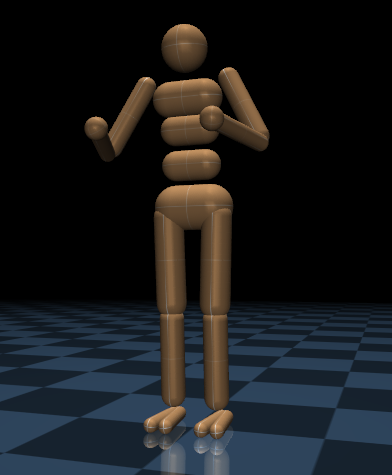
\includegraphics[scale=0.8]{humanoid.png}
            \caption{Humanoide do ambiente virtual \textit{Mujoco}.}
            % http://www.mujoco.org/forum/index.php?attachments/humanoid-png.48/
        \end{figure}

    \section{Implementações em DRL}

        Após estudos introdutórios acerca do tema, decidimos
        que seria interessante aplicá-los. Realizei os exercícios
        disponibilizados pela \textit{UC Berkeley} para \textit{Reinforcement
        Learning}
        % http://ai.berkeley.edu/reinforcement.html
        , sendo que o último deles é a implementação para o jogo
        do \textit{Pac-Man}, buscando "ensinar"\ o personagem para que
        ele vença o jogo sozinho.

        \begin{figure}[h!]
            \centering
            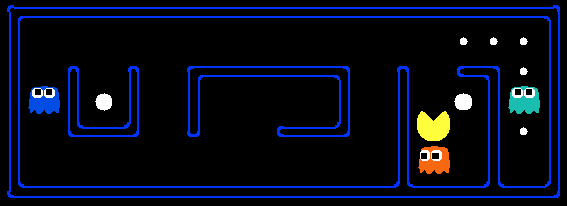
\includegraphics[width=\textwidth]{pac_man.png}
            \caption{\textit{Pac-Man}.}
            % http://ai.berkeley.edu/projects/release/reinforcement/v1/001/capsule.png
        \end{figure}

        Foi muito conveniente também a implementação de vários dos 
        algoritmos de \textit{Reinforcement Learning} agregados em
        % https://medium.com/@m.alzantot/deep-reinforcement-learning-demysitifed-episode-2-policy-iteration-value-iteration-and-q-978f9e89ddaa
        , utilizando os ambientes da biblioteca para \textit{Reinforcement Learning} chamada \textit{Gym}.
        Utilizando esses ambientes, como o da Figura \ref{fig:mountaincar-v0}, é, em geral, treinar
        o personagem para realizar uma tarefa.
        O algoritmo de \textit{Q-learning} foi um desses algoritmos.
        A base desse algoritmo é uma tabela,
        utilizada para tentar aproximar uma função. Substituindo essa tabela por
        uma rede neural (para executar uma mesma função), o resultado fica muito
        legal também. Os códigos podem ser conferidos no meu repositório no \textit{GitHub}
        % https://github.com/lucasresck/deep-reinforcement-learning.

        \begin{figure}[h!]
            \centering
            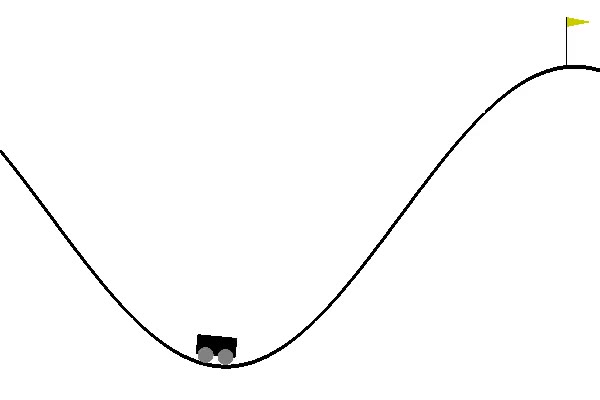
\includegraphics[width=\textwidth]{mountaincar_v0.jpg}
            \caption{Ambiente \textit{MountainCar-v0} da biblioteca \textit{Gym}.
            O objetivo nesse ambiente é fazer o carrinho chegar ao topo da montanha.}
            % https://gym.openai.com/videos/2019-10-21--mqt8Qj1mwo/MountainCar-v0/poster.jpg
            \label{fig:mountaincar-v0}
        \end{figure}

    \section{Visualização na Web}

    \section{Futuras extensões}

    \bibliographystyle{plain}
    \bibliography{references}
\end{document}
